
%% bare_conf.tex
%% V1.3
%% 2007/01/11
%% by Michael Shell
%% See:
%% http://www.michaelshell.org/
%% for current contact information.
%%
%% This is a skeleton file demonstrating the use of IEEEtran.cls
%% (requires IEEEtran.cls version 1.7 or later) with an IEEE conference paper.
%%
%% Support sites:
%% http://www.michaelshell.org/tex/ieeetran/
%% http://www.ctan.org/tex-archive/macros/latex/contrib/IEEEtran/
%% and
%% http://www.ieee.org/

%%*************************************************************************
%% Legal Notice:
%% This code is offered as-is without any warranty either expressed or
%% implied; without even the implied warranty of MERCHANTABILITY or
%% FITNESS FOR A PARTICULAR PURPOSE! 
%% User assumes all risk.
%% In no event shall IEEE or any contributor to this code be liable for
%% any damages or losses, including, but not limited to, incidental,
%% consequential, or any other damages, resulting from the use or misuse
%% of any information contained here.
%%
%% All comments are the opinions of their respective authors and are not
%% necessarily endorsed by the IEEE.
%%
%% This work is distributed under the LaTeX Project Public License (LPPL)
%% ( http://www.latex-project.org/ ) version 1.3, and may be freely used,
%% distributed and modified. A copy of the LPPL, version 1.3, is included
%% in the base LaTeX documentation of all distributions of LaTeX released
%% 2003/12/01 or later.
%% Retain all contribution notices and credits.
%% ** Modified files should be clearly indicated as such, including  **
%% ** renaming them and changing author support contact information. **
%%
%% File list of work: IEEEtran.cls, IEEEtran_HOWTO.pdf, bare_adv.tex,
%%                    bare_conf.tex, bare_jrnl.tex, bare_jrnl_compsoc.tex
%%*************************************************************************

% *** Authors should verify (and, if needed, correct) their LaTeX system  ***
% *** with the testflow diagnostic prior to trusting their LaTeX platform ***
% *** with production work. IEEE's font choices can trigger bugs that do  ***
% *** not appear when using other class files.                            ***
% The testflow support page is at:
% http://www.michaelshell.org/tex/testflow/



% Note that the a4paper option is mainly intended so that authors in
% countries using A4 can easily print to A4 and see how their papers will
% look in print - the typesetting of the document will not typically be
% affected with changes in paper size (but the bottom and side margins will).
% Use the testflow package mentioned above to verify correct handling of
% both paper sizes by the user's LaTeX system.
%
% Also note that the "draftcls" or "draftclsnofoot", not "draft", option
% should be used if it is desired that the figures are to be displayed in
% draft mode.
%
\documentclass[conference]{IEEEtran}
% Add the compsoc option for Computer Society conferences.
%
% If IEEEtran.cls has not been installed into the LaTeX system files,
% manually specify the path to it like:
% \documentclass[conference]{../sty/IEEEtran}





% Some very useful LaTeX packages include:
% (uncomment the ones you want to load)


% *** MISC UTILITY PACKAGES ***
%
%\usepackage{ifpdf}
% Heiko Oberdiek's ifpdf.sty is very useful if you need conditional
% compilation based on whether the output is pdf or dvi.
% usage:
% \ifpdf
%   % pdf code
% \else
%   % dvi code
% \fi
% The latest version of ifpdf.sty can be obtained from:
% http://www.ctan.org/tex-archive/macros/latex/contrib/oberdiek/
% Also, note that IEEEtran.cls V1.7 and later provides a builtin
% \ifCLASSINFOpdf conditional that works the same way.
% When switching from latex to pdflatex and vice-versa, the compiler may
% have to be run twice to clear warning/error messages.






% *** CITATION PACKAGES ***
%
%\usepackage{cite}
% cite.sty was written by Donald Arseneau
% V1.6 and later of IEEEtran pre-defines the format of the cite.sty package
% \cite{} output to follow that of IEEE. Loading the cite package will
% result in citation numbers being automatically sorted and properly
% "compressed/ranged". e.g., [1], [9], [2], [7], [5], [6] without using
% cite.sty will become [1], [2], [5]--[7], [9] using cite.sty. cite.sty's
% \cite will automatically add leading space, if needed. Use cite.sty's
% noadjust option (cite.sty V3.8 and later) if you want to turn this off.
% cite.sty is already installed on most LaTeX systems. Be sure and use
% version 4.0 (2003-05-27) and later if using hyperref.sty. cite.sty does
% not currently provide for hyperlinked citations.
% The latest version can be obtained at:
% http://www.ctan.org/tex-archive/macros/latex/contrib/cite/
% The documentation is contained in the cite.sty file itself.






% *** GRAPHICS RELATED PACKAGES ***
%
\ifCLASSINFOpdf
  % \usepackage[pdftex]{graphicx}
  % declare the path(s) where your graphic files are
  % \graphicspath{{../pdf/}{../jpeg/}}
  % and their extensions so you won't have to specify these with
  % every instance of \includegraphics
  % \DeclareGraphicsExtensions{.pdf,.jpeg,.png}
\else
  % or other class option (dvipsone, dvipdf, if not using dvips). graphicx
  % will default to the driver specified in the system graphics.cfg if no
  % driver is specified.
  % \usepackage[dvips]{graphicx}
  % declare the path(s) where your graphic files are
  % \graphicspath{{../eps/}}
  % and their extensions so you won't have to specify these with
  % every instance of \includegraphics
  % \DeclareGraphicsExtensions{.eps}
\fi
% graphicx was written by David Carlisle and Sebastian Rahtz. It is
% required if you want graphics, photos, etc. graphicx.sty is already
% installed on most LaTeX systems. The latest version and documentation can
% be obtained at: 
% http://www.ctan.org/tex-archive/macros/latex/required/graphics/
% Another good source of documentation is "Using Imported Graphics in
% LaTeX2e" by Keith Reckdahl which can be found as epslatex.ps or
% epslatex.pdf at: http://www.ctan.org/tex-archive/info/
%
% latex, and pdflatex in dvi mode, support graphics in encapsulated
% postscript (.eps) format. pdflatex in pdf mode supports graphics
% in .pdf, .jpeg, .png and .mps (metapost) formats. Users should ensure
% that all non-photo figures use a vector format (.eps, .pdf, .mps) and
% not a bitmapped formats (.jpeg, .png). IEEE frowns on bitmapped formats
% which can result in "jaggedy"/blurry rendering of lines and letters as
% well as large increases in file sizes.
%
% You can find documentation about the pdfTeX application at:
% http://www.tug.org/applications/pdftex





% *** MATH PACKAGES ***
%
%\usepackage[cmex10]{amsmath}
% A popular package from the American Mathematical Society that provides
% many useful and powerful commands for dealing with mathematics. If using
% it, be sure to load this package with the cmex10 option to ensure that
% only type 1 fonts will utilized at all point sizes. Without this option,
% it is possible that some math symbols, particularly those within
% footnotes, will be rendered in bitmap form which will result in a
% document that can not be IEEE Xplore compliant!
%
% Also, note that the amsmath package sets \interdisplaylinepenalty to 10000
% thus preventing page breaks from occurring within multiline equations. Use:
%\interdisplaylinepenalty=2500
% after loading amsmath to restore such page breaks as IEEEtran.cls normally
% does. amsmath.sty is already installed on most LaTeX systems. The latest
% version and documentation can be obtained at:
% http://www.ctan.org/tex-archive/macros/latex/required/amslatex/math/





% *** SPECIALIZED LIST PACKAGES ***
%
%\usepackage{algorithmic}
% algorithmic.sty was written by Peter Williams and Rogerio Brito.
% This package provides an algorithmic environment fo describing algorithms.
% You can use the algorithmic environment in-text or within a figure
% environment to provide for a floating algorithm. Do NOT use the algorithm
% floating environment provided by algorithm.sty (by the same authors) or
% algorithm2e.sty (by Christophe Fiorio) as IEEE does not use dedicated
% algorithm float types and packages that provide these will not provide
% correct IEEE style captions. The latest version and documentation of
% algorithmic.sty can be obtained at:
% http://www.ctan.org/tex-archive/macros/latex/contrib/algorithms/
% There is also a support site at:
% http://algorithms.berlios.de/index.html
% Also of interest may be the (relatively newer and more customizable)
% algorithmicx.sty package by Szasz Janos:
% http://www.ctan.org/tex-archive/macros/latex/contrib/algorithmicx/




% *** ALIGNMENT PACKAGES ***
%
%\usepackage{array}
% Frank Mittelbach's and David Carlisle's array.sty patches and improves
% the standard LaTeX2e array and tabular environments to provide better
% appearance and additional user controls. As the default LaTeX2e table
% generation code is lacking to the point of almost being broken with
% respect to the quality of the end results, all users are strongly
% advised to use an enhanced (at the very least that provided by array.sty)
% set of table tools. array.sty is already installed on most systems. The
% latest version and documentation can be obtained at:
% http://www.ctan.org/tex-archive/macros/latex/required/tools/


%\usepackage{mdwmath}
%\usepackage{mdwtab}
% Also highly recommended is Mark Wooding's extremely powerful MDW tools,
% especially mdwmath.sty and mdwtab.sty which are used to format equations
% and tables, respectively. The MDWtools set is already installed on most
% LaTeX systems. The lastest version and documentation is available at:
% http://www.ctan.org/tex-archive/macros/latex/contrib/mdwtools/


% IEEEtran contains the IEEEeqnarray family of commands that can be used to
% generate multiline equations as well as matrices, tables, etc., of high
% quality.


%\usepackage{eqparbox}
% Also of notable interest is Scott Pakin's eqparbox package for creating
% (automatically sized) equal width boxes - aka "natural width parboxes".
% Available at:
% http://www.ctan.org/tex-archive/macros/latex/contrib/eqparbox/





% *** SUBFIGURE PACKAGES ***
%\usepackage[tight,footnotesize]{subfigure}
% subfigure.sty was written by Steven Douglas Cochran. This package makes it
% easy to put subfigures in your figures. e.g., "Figure 1a and 1b". For IEEE
% work, it is a good idea to load it with the tight package option to reduce
% the amount of white space around the subfigures. subfigure.sty is already
% installed on most LaTeX systems. The latest version and documentation can
% be obtained at:
% http://www.ctan.org/tex-archive/obsolete/macros/latex/contrib/subfigure/
% subfigure.sty has been superceeded by subfig.sty.



%\usepackage[caption=false]{caption}
%\usepackage[font=footnotesize]{subfig}
% subfig.sty, also written by Steven Douglas Cochran, is the modern
% replacement for subfigure.sty. However, subfig.sty requires and
% automatically loads Axel Sommerfeldt's caption.sty which will override
% IEEEtran.cls handling of captions and this will result in nonIEEE style
% figure/table captions. To prevent this problem, be sure and preload
% caption.sty with its "caption=false" package option. This is will preserve
% IEEEtran.cls handing of captions. Version 1.3 (2005/06/28) and later 
% (recommended due to many improvements over 1.2) of subfig.sty supports
% the caption=false option directly:
%\usepackage[caption=false,font=footnotesize]{subfig}
%
% The latest version and documentation can be obtained at:
% http://www.ctan.org/tex-archive/macros/latex/contrib/subfig/
% The latest version and documentation of caption.sty can be obtained at:
% http://www.ctan.org/tex-archive/macros/latex/contrib/caption/




% *** FLOAT PACKAGES ***
%
%\usepackage{fixltx2e}
% fixltx2e, the successor to the earlier fix2col.sty, was written by
% Frank Mittelbach and David Carlisle. This package corrects a few problems
% in the LaTeX2e kernel, the most notable of which is that in current
% LaTeX2e releases, the ordering of single and double column floats is not
% guaranteed to be preserved. Thus, an unpatched LaTeX2e can allow a
% single column figure to be placed prior to an earlier double column
% figure. The latest version and documentation can be found at:
% http://www.ctan.org/tex-archive/macros/latex/base/



%\usepackage{stfloats}
% stfloats.sty was written by Sigitas Tolusis. This package gives LaTeX2e
% the ability to do double column floats at the bottom of the page as well
% as the top. (e.g., "\begin{figure*}[!b]" is not normally possible in
% LaTeX2e). It also provides a command:
%\fnbelowfloat
% to enable the placement of footnotes below bottom floats (the standard
% LaTeX2e kernel puts them above bottom floats). This is an invasive package
% which rewrites many portions of the LaTeX2e float routines. It may not work
% with other packages that modify the LaTeX2e float routines. The latest
% version and documentation can be obtained at:
% http://www.ctan.org/tex-archive/macros/latex/contrib/sttools/
% Documentation is contained in the stfloats.sty comments as well as in the
% presfull.pdf file. Do not use the stfloats baselinefloat ability as IEEE
% does not allow \baselineskip to stretch. Authors submitting work to the
% IEEE should note that IEEE rarely uses double column equations and
% that authors should try to avoid such use. Do not be tempted to use the
% cuted.sty or midfloat.sty packages (also by Sigitas Tolusis) as IEEE does
% not format its papers in such ways.





% *** PDF, URL AND HYPERLINK PACKAGES ***
%
%\usepackage{url}
% url.sty was written by Donald Arseneau. It provides better support for
% handling and breaking URLs. url.sty is already installed on most LaTeX
% systems. The latest version can be obtained at:
% http://www.ctan.org/tex-archive/macros/latex/contrib/misc/
% Read the url.sty source comments for usage information. Basically,
% \url{my_url_here}.





% *** Do not adjust lengths that control margins, column widths, etc. ***
% *** Do not use packages that alter fonts (such as pslatex).         ***
% There should be no need to do such things with IEEEtran.cls V1.6 and later.
% (Unless specifically asked to do so by the journal or conference you plan
% to submit to, of course. )


% correct bad hyphenation here
\hyphenation{op-tical net-works semi-conduc-tor}


\begin{document}
%
% paper title
% can use linebreaks \\ within to get better formatting as desired
\title{Bare Demo of IEEEtran.cls for Conferences}


% author names and affiliations
% use a multiple column layout for up to three different
% affiliations
\author{\IEEEauthorblockN{Michael Shell}
\IEEEauthorblockA{School of Electrical and\\Computer Engineering\\
Georgia Institute of Technology\\
Atlanta, Georgia 30332--0250\\
Email: http://www.michaelshell.org/contact.html}
\and
\IEEEauthorblockN{Homer Simpson}
\IEEEauthorblockA{Twentieth Century Fox\\
Springfield, USA\\
Email: homer@thesimpsons.com}
\and
\IEEEauthorblockN{James Kirk\\ and Montgomery Scott}
\IEEEauthorblockA{Starfleet Academy\\
San Francisco, California 96678-2391\\
Telephone: (800) 555--1212\\
Fax: (888) 555--1212}}

% conference papers do not typically use \thanks and this command
% is locked out in conference mode. If really needed, such as for
% the acknowledgment of grants, issue a \IEEEoverridecommandlockouts
% after \documentclass

% for over three affiliations, or if they all won't fit within the width
% of the page, use this alternative format:
% 
%\author{\IEEEauthorblockN{Michael Shell\IEEEauthorrefmark{1},
%Homer Simpson\IEEEauthorrefmark{2},
%James Kirk\IEEEauthorrefmark{3}, 
%Montgomery Scott\IEEEauthorrefmark{3} and
%Eldon Tyrell\IEEEauthorrefmark{4}}
%\IEEEauthorblockA{\IEEEauthorrefmark{1}School of Electrical and Computer Engineering\\
%Georgia Institute of Technology,
%Atlanta, Georgia 30332--0250\\ Email: see http://www.michaelshell.org/contact.html}
%\IEEEauthorblockA{\IEEEauthorrefmark{2}Twentieth Century Fox, Springfield, USA\\
%Email: homer@thesimpsons.com}
%\IEEEauthorblockA{\IEEEauthorrefmark{3}Starfleet Academy, San Francisco, California 96678-2391\\
%Telephone: (800) 555--1212, Fax: (888) 555--1212}
%\IEEEauthorblockA{\IEEEauthorrefmark{4}Tyrell Inc., 123 Replicant Street, Los Angeles, California 90210--4321}}




% use for special paper notices
%\IEEEspecialpapernotice{(Invited Paper)}




% make the title area
\maketitle


\begin{abstract}
%\boldmath
The abstract goes here.
\end{abstract}
% IEEEtran.cls defaults to using nonbold math in the Abstract.
% This preserves the distinction between vectors and scalars. However,
% if the conference you are submitting to favors bold math in the abstract,
% then you can use LaTeX's standard command \boldmath at the very start
% of the abstract to achieve this. Many IEEE journals/conferences frown on
% math in the abstract anyway.

% no keywords




% For peer review papers, you can put extra information on the cover
% page as needed:
% \ifCLASSOPTIONpeerreview
% \begin{center} \bfseries EDICS Category: 3-BBND \end{center}
% \fi
%
% For peerreview papers, this IEEEtran command inserts a page break and
% creates the second title. It will be ignored for other modes.
\IEEEpeerreviewmaketitle

\section{Motivation}
Technical debt is a metaphor in which the consequences of decisions that affect the maintenance of a software system, such as decisions regarding architecture and code structure, are described with attributes of financial debt~\cite{Cunningham:1992}. Economic models proposed by the \TD community quantify debt using the concepts of principal and interest, where principal is the cost to repay the debt by reworking the code and interest is the cost accumulated by developers working around the debt while the principal is not repaid.

Several approaches for estimating principal are based on heuristics that use measures of structural code quality as inputs to models that estimate effort. For example, Nugroho et al.~\cite{Nugroho_etal:2011} provide a model for estimating principal using maintainability ratings based on measures obtained via static analysis of code, and a model for estimating interest using estimates of maintenance effort based on change history of code. Curtis \etal~\cite{Curtis_etal:2012} also provide a model for estimating principal using measures based on static analysis of code, but in their model, principal is a function of the number of problems, the time/effort required to fix each problem, and the cost of fixing a problem.
\Fix{Will:\TD is not just code structure related}

Although such models provide the means to estimate debt, it may be difficult to justify reducing technical debt without detailed information about the impact of the debt on developer's day-to-day maintenance activities. Until the debt reaches a point at which it has a substantial impact on the progress or cost of maintenance, developers may be forced to work around areas of the code in which the debt is manifest~\cite{Ozkaya_etal:2011}. 
Because most developer effort during software maintenance is spent on program comprehension activities such as reading and navigating code~\cite{Fjeldstad_Hamlen:1982,Standish:1984,vonMayrhauser_etal:1997,Ko_etal:2006,LaToza_etal:2006,Tiarks:2011}, understanding the impact of structural-quality-related debt on code comprehension is of critical importance. In this paper, we propose a framework to support continuous estimation of interest payments on technical debt by monitoring the effort that developers must expend to comprehend code as they complete change tasks. 

In our proposed framework, principal estimation is based on measures of code maintainability obtained via static analysis, and interest estimation is based on activity data obtained by monitoring developer actions in the IDE. Our monitoring tool, $Blaze$~\cite{Snipes_etal:2014}, records a temporal sequence of developer actions, including code navigation actions and edit actions, in a log. We analyze this log to understand class relationships and to quantify the effort spent by a developer to comprehend individual program elements while completing a change task. By combining this comprehension effort data with the code maintainability measurements, we can provide evidence of how \TD impacts developer-code-comprehension effort and continuously update interest payment estimates.
\Fix{Will:this sentence was unclear}

% no \IEEEPARstart
\section{Objectives}
%\input{ObjectivesForMeasrement}

\section{Data}
%In this section we define the specific measurements, data analysis and relationships for the framework to to meet the objectives of quantifying comprehension effort as related to interest payments on technical debt.

Data for calculating the comprehension effort for developers comes from the $Blaze$~\cite{Snipes_etal:2014} monitoring tool.  $Blaze$ logs events anonymously from developer actions in Visual Studio including menu commands, shortcut-keys, and source code editor actions such as moving the insertion carat and scrolling.  Developers at ABB volunteered to install $Blaze$ and record their actions in Visual Studio.  The data set evaluated for this study focuses on two developers with more than 3 months of data.  Table~\ref{fig:SampleEventData} shows a sample of the log data where each row contains a date and time (date not shown) for the event, a unique ID anonymously assigned to the developer, the event name recorded from Visual Studio, and a reference to the source file and location within the file.

\begin{table}[!t]
\renewcommand{\arraystretch}{1.3}
\centering
	\caption{Sample Data From Event Log}
	\begin{tabular}{llll}
	\toprule
\textbf{Time-stamp} & \textbf{User} & \textbf{Event} & \textbf{Artifact} \\
\midrule
22:04:51 & N3 & View.SourceFile & 1acc7366.cs/10 \\
22:04:52 & N3 & View.OnChangeCaretLine & 1acc7366.cs/14 \\
22:04:53 & N3 & View.OnChangeCaretLine & 1acc7366.cs/16 \\
22:04:58 & N3 & Menu.ViewCallHierarchy & 1acc7366.cs/16 \\
22:05:00 & N3 & View.OnChangeCaretLine & 1acc7366.cs/20 \\
22:05:19 & N3 & View.SourceFile & 81c2db1a.cs/1 \\
22:05:22 & N3 & Edit.Find & 81c2db1a.cs/1 \\
22:05:30 & N3 & Edit.FindNext & 81c2db1a.cs/20 \\
\bottomrule
	\end{tabular}
%	\includegraphics[width=2.75in]{figures/SampleEventData.pdf}
	\label{fig:SampleEventData}
\end{table}

Measuring comprehension effort from $Blaze$ monitoring logs requires extracting development sessions from the data that segment the stream of activity into periods where the developer is focused on a particular class.  We define a session as fixed length time window where the developer is investigating a certain class we call the central class.  The session time window begins with the first time the developer visits a certain class and ends with the last occurrence of a visit to the class within the fixed length time window.  The length of the time window is a variable we investigate in Section \ref{sec:AnalysisResults}.  
\Comment{Will:I think the previous 3 sentences define what we call a super block in our discussions}
\Fix{Will:See AnalysisResults question about number of sessions and consider moving the paragraph with that information here.}

In Figure \ref{fig:SessionDataConcept} we show the session concept.  The session starts with the first visit to Class A under the green circle.  After that other classes C and E are visited including a visit to Class A again before the last visit to Class A under the red hexagon.  After the last visit the session time window expires.  The next session starts with a visit to Class A that begins a new 4 hour window.  In this visit classes C and E are visited as well before the developer returns to Class A.  Thus you see there are two sessions for Class A which contain a total of five visits to Class A, three visits to Class C and two visits to Class E.
\begin{figure}
	\centering
	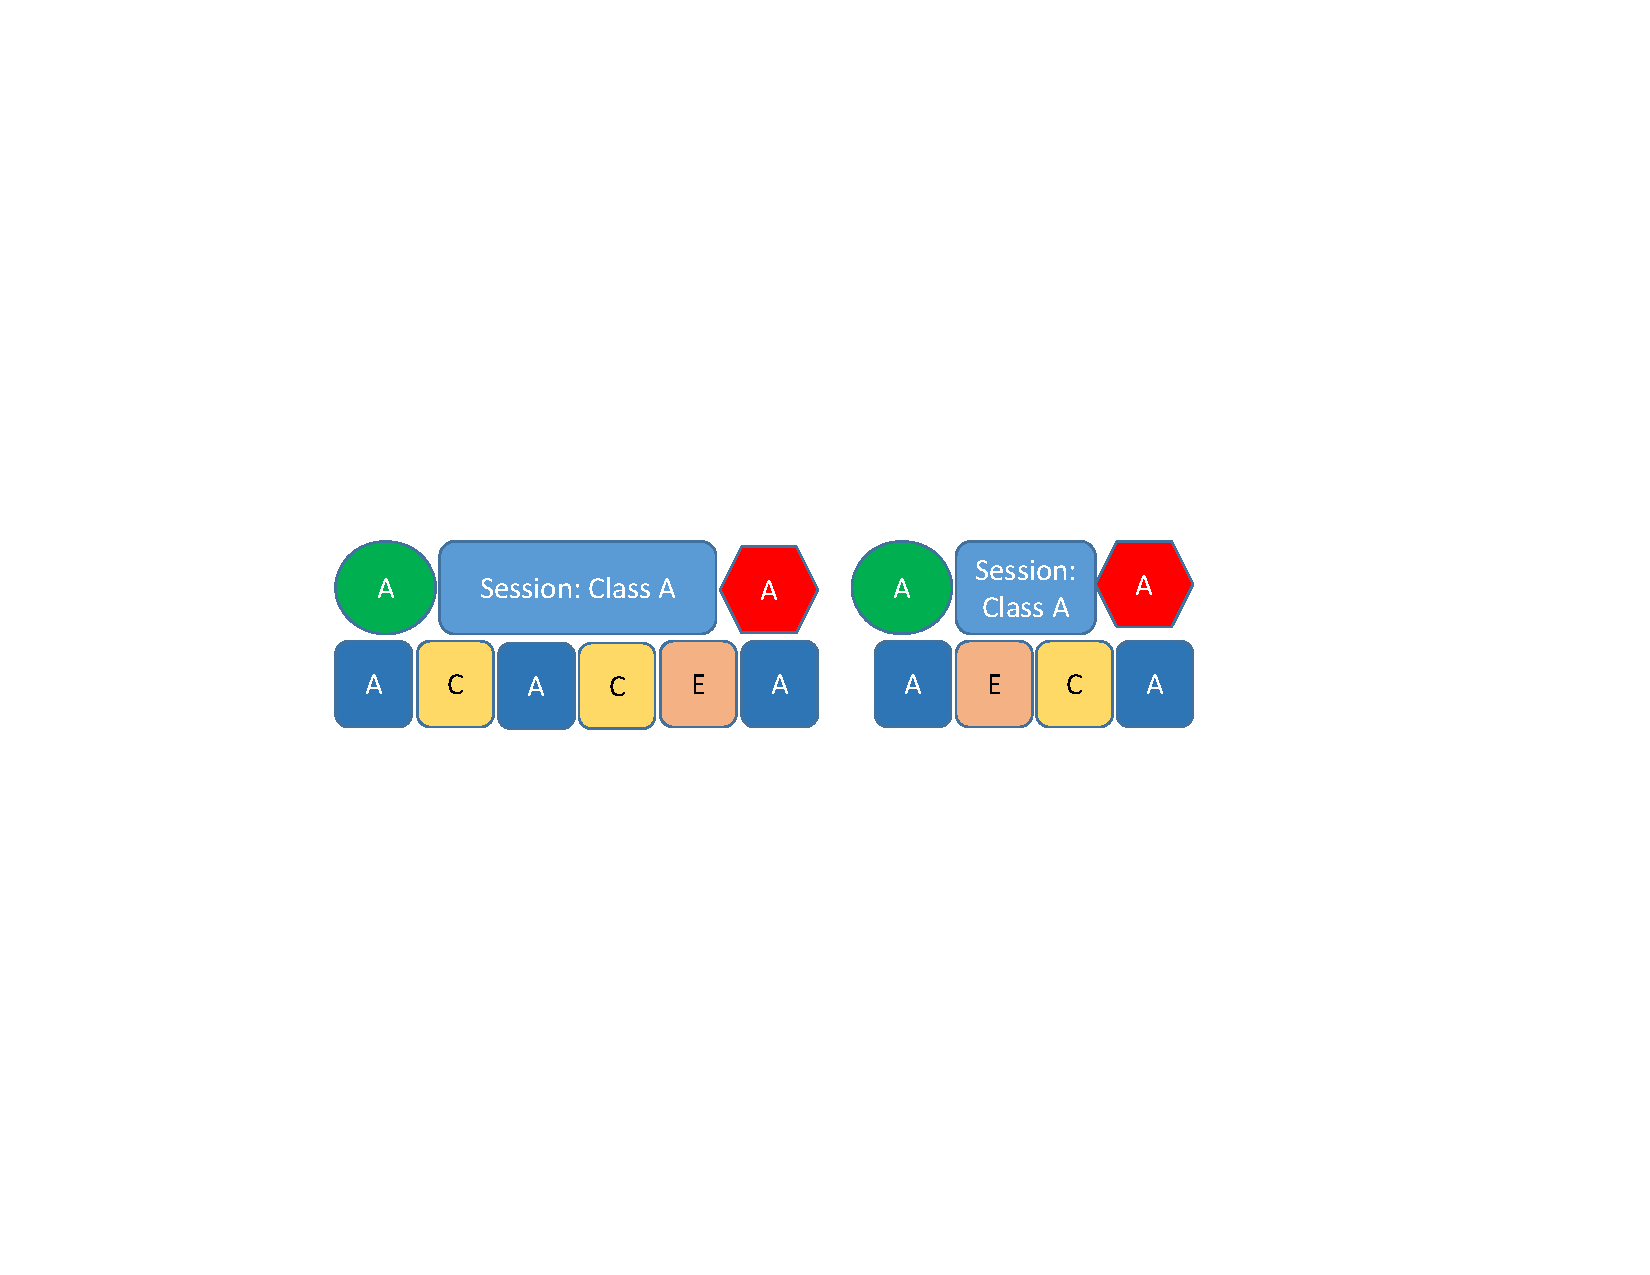
\includegraphics[width=\linewidth]{SessionDataConcept.pdf}
	\caption{Conceptual View of Sessions}
	\label{fig:SessionDataConcept}
\end{figure}

\Fix{The following is unclear in the context of block and super block}
When sessions repeat, additional or fewer classes may be viewed by the developer, regardless they incur some comprehension effort which we add to the interest payments.  In each session, we determine the interest amount from the comprehension data quantifying it in hours. 


Within a session, we calculate measurements related to comprehension effort as follows:
\begin{itemize}
	\item[] $Number of sessions$ is the number of time window sessions formed by each class 
	\item[] $Count Number of Class Visits$ is the number of times the class itself has been accessed inside a session \Fix{Will:changed Edits to Visits..I think we mean visits?}
	\item[] $Count Number of Other Class Accesses$ is the number of unique files visited in each session
	\item[] $Time Spent in Class$ is the time spent in the class that forms the session
	\item[] $Time Spent in Other Classes$ is the time spent in all other files in the session
\end{itemize}

  

The framework matches the comprehension data with code structure data at the class level.  Therefore we consider class level code structure metrics whose definitions align with the measurements taken for comprehension.  Data for code structure is provided by the $Understand$ tool from Scientific Tool Works.  The framework used the following metrics for code structure data at the class level:

\begin{itemize}
	\item[] $Count Class Coupled$ is the number of other classes coupled to
	\item[] $Count Class Base$ is the Number of immediate base classes
	\item[] $Count Class Derived$ is the number of immediate sub-classes
	\item[] $Count Declared Method$ is the number of local methods for the class
\end{itemize}

The class level metrics for code structure are related to comprehension metrics through the name of the source file in the $Blaze$ data corresponding to the class.  In cases where the source file contains multiple classes, the structure metrics were aggregated.

Aligning these two data sources at the module level allows us to ask questions of the intersected data set.  For example, we find the following questions interesting:

\begin{itemize}
	\item[] How much time does the developer spend understanding the code related to the change they are making?
	\item[] How many code elements does the developer need to review related to the change?
	\item[] How many dependent classes does the developer need to review related to the change?
	\item[] How correlated are comprehension effort metrics with code structure metrics?
	\item[] As code structure metic values change, is the corresponding change in comprehension effort linear or non-linear.
\end{itemize}

\section{Analysis}
%\begin{center}
\begin{table*}[t]
	\centering
	\caption{Class Data for Each Developer}
	\begin{tabular}{|l|l|l|l|l|l|l|}
	\hline

Developer Name & Class Name & No Of Blocks &Count No of Class Edits & Count No of Other Class Accesses & Time Spent in Class & Time Spent in Other Classes\\
\hline\hline
Developer X & A & 74 & 294 & 78 & 39hours 34mins 23 secs & 16hours 39mins 36secs\\
\hline
Developer X & B & 32 & 88 & 52 & 2hours 54mins 20 secs & 8hours 54mins 18secs\\
\hline
Developer X & C & 28 & 77 & 52 & 4hours 28mins 25 secs & 9hours 15mins 41secs\\
\hline
Developer Y & P & 10 & 45 & 24 & 2hours 19mins 13 secs & 1hour 43mins 12secs\\
\hline
Developer Y & Q & 7 & 12 & 20 & 24 mins 08 secs & 2hours 36mins 32secs\\
\hline
Developer Y & R & 5 & 15 & 16 & 53 mins 51 secs & 40mins 18secs\\
\hline

	\end{tabular}
	\label{fig:AnalysisData}
\end{table*}
\end{center}

As previously mentioned we first define sessions to investigate each class that a developer visits. We define session as a moving window time where developer is investigating a certain class. When we define a session of X hours for a class Y we mean to say that starting from the first time the developer visits class Y while navigating we find the last time he visits the same class in X hours. We refer to this unit as a  "block" for the class that we want to study. For each block of class Y that we obtain we study the number of unique classes the developer has visited while in the block as well as the number of times the developer has visited the class Y iteslf within the block. The classes central to a task will have a high count of the number of times the developer visits the class in a particular block and the number of such blocks will also be high. We also calculate the time spent by developer in the central class as well as the time spent by the developer spent in other classes in the block of the central class.The time factor gives us an estimation of how well the developer comprehends the class and other classes referenced in the block. We studied such blocks for a moving window of 4 hours, 8 hours, 12 hours and 16 hours. 

The data collected by the Blaze logs has all the navigation activities done by the developer in the IDE. It also has appropriate time outs for periods of inactivity in the IDE. We first filtered out all the navigation activities related to classes as well all time outs and IDE exits. Next we calculated the time spent by the developer in the class. We obtained a list of such classes and the time spent by the user in each class. We observed there were instances when the developer accessed a class for less than a second and then switched to another class. We assumed that no useful comprehension can be done by the user in less than a second and attributed such class accesses to random clicks and removed all such entries. We then calculated various parameters that would help in identifying the central class as well the neccesary classes for comprehending the central class. For each sliding window size we calculated the following parameters:
\begin{itemize}
	\item[] Number of blocks formed by each class (No Of Blocks).
	\item[] Number of times the class itself has been accessed inside the block (Count No of Class Edits).
	\item[] Number of unique files visited in each block (Count No of Other Class Accesses).
	\item[] Time spent in the class that forms the block (Time Spent in Class).
	\item[] Time spent in all other files in the block (Time Spent in Other Classes). 
\end{itemize}
We observed that there was a small change in the number of blocks formed by each class between the 4 hour moving window and the 8 hour moving window. The fact that there is not a huge downslide from the 4 hour window to the 8 hour window means that developers do not very often work in 8 hour windows but rather more often do so in 4 hour windows. The 8 hour moving window formed the same number of blocks as that of the 12 hour and 16 hour window. Since the difference was not much between the 4 hour and 8 hour sliding window we decided to use the 4 hour sliding window for further analysis.

Table~\ref{fig:AnalysisData} shows data for each developer that we investigated. We present 3 classes for each of the developers. Each column represents the 5 parameters we defined to be useful in quantifying the \TD. As you can see for developer X we observe a very high count of the number of blocks as well as high counts in number of class edits and number of other class accesses for Class A. This suggests that the developer referenced Class A over a long period of time and very frequently. The developer also frequently referred to other classes while working on Class A. The data shows that the developer spent more than 39 hours working on Class A and more than 16 hours referencing other classes. The 16 hours the developer spent on other files can be interpreted as a cost of comprehending class A. Thus it can be veiwed as  \TD. Similarly when we see Class B we see that developer X spent nearly 3 hours on Class B but spent nearly 9 hours referencing other classes. This indicates that the developer spent 3 times the time actually spent on the central class in other classes. Only taking time as a factor cannot lead to such conclusions and we need to make sure that the class that we consider as the block is central to the task at hand. In this case the developer has 32 such blocks of Class B where he has also referenced Class B 88 times in these blocks. We can safely say that the developer keeps coming back to class B and thus it must be central to the task. Similar patterns can be seen in developer Y where each parameter is indicative of the fact that the considered class is indeed the central class and that the time spent navigating other classes has a significant impact in calculating \TD.


\section{Conclusions and Future Ideas}
In this paper we proposed a framework in which code maintainability data and comprehension effort data are combined to support continuous updates of interest payment estimates, which in turn supports real-time prioritization of debt removal efforts. The primary contribution of our proposed framework is the integration of developer activity data with static code metrics and the concomitant improvements in understanding of developer comprehension effort and in the accuracy with which interest payments can be estimated. An initial investigation of data that we collected from ABB developers demonstrates the feasibility of the framework and provides examples of how the developer activity data work in concert with structural code metrics to reveal new information about developer comprehension effort.

Our next step will be to conduct a large-scale statistical analysis of comprehension and structural metrics to better understand the correlations and levels of technical debt that drive increased comprehension effort.  With this analysis we will determine how to calculate interest payments for technical debt items.  This will include resolving what portion of comprehension effort is for technical debt and the portion that is inherent in comprehending the ideal code structure.  

We plan to further develop the framework and to use it to answer a number of questions about the relationships between developer comprehension effort and technical debt.  For example, we plan to include other comprehension metrics such as the number of edits to a class that will allow evaluation of the Shotgun Surgery smell where multiple classes are modified for a change.  To improve the accuracy of the comprehension data, we plan to detect the central class based on edit actions as well as navigation and search actions during a session.  We also plan to conduct an observational study of developers to validate the estimates  of interest payments during maintenance activities.



% An example of a floating figure using the graphicx package.
% Note that \label must occur AFTER (or within) \caption.
% For figures, \caption should occur after the \includegraphics.
% Note that IEEEtran v1.7 and later has special internal code that
% is designed to preserve the operation of \label within \caption
% even when the captionsoff option is in effect. However, because
% of issues like this, it may be the safest practice to put all your
% \label just after \caption rather than within \caption{}.
%
% Reminder: the "draftcls" or "draftclsnofoot", not "draft", class
% option should be used if it is desired that the figures are to be
% displayed while in draft mode.
%
%\begin{figure}[!t]
%\centering
%\includegraphics[width=2.5in]{myfigure}
% where an .eps filename suffix will be assumed under latex, 
% and a .pdf suffix will be assumed for pdflatex; or what has been declared
% via \DeclareGraphicsExtensions.
%\caption{Simulation Results}
%\label{fig_sim}
%\end{figure}

% Note that IEEE typically puts floats only at the top, even when this
% results in a large percentage of a column being occupied by floats.


% An example of a double column floating figure using two subfigures.
% (The subfig.sty package must be loaded for this to work.)
% The subfigure \label commands are set within each subfloat command, the
% \label for the overall figure must come after \caption.
% \hfil must be used as a separator to get equal spacing.
% The subfigure.sty package works much the same way, except \subfigure is
% used instead of \subfloat.
%
%\begin{figure*}[!t]
%\centerline{\subfloat[Case I]\includegraphics[width=2.5in]{subfigcase1}%
%\label{fig_first_case}}
%\hfil
%\subfloat[Case II]{\includegraphics[width=2.5in]{subfigcase2}%
%\label{fig_second_case}}}
%\caption{Simulation results}
%\label{fig_sim}
%\end{figure*}
%
% Note that often IEEE papers with subfigures do not employ subfigure
% captions (using the optional argument to \subfloat), but instead will
% reference/describe all of them (a), (b), etc., within the main caption.


% An example of a floating table. Note that, for IEEE style tables, the 
% \caption command should come BEFORE the table. Table text will default to
% \footnotesize as IEEE normally uses this smaller font for tables.
% The \label must come after \caption as always.
%
%\begin{table}[!t]
%% increase table row spacing, adjust to taste
%\renewcommand{\arraystretch}{1.3}
% if using array.sty, it might be a good idea to tweak the value of
% \extrarowheight as needed to properly center the text within the cells
%\caption{An Example of a Table}
%\label{table_example}
%\centering
%% Some packages, such as MDW tools, offer better commands for making tables
%% than the plain LaTeX2e tabular which is used here.
%\begin{tabular}{|c||c|}
%\hline
%One & Two\\
%\hline
%Three & Four\\
%\hline
%\end{tabular}
%\end{table}


% Note that IEEE does not put floats in the very first column - or typically
% anywhere on the first page for that matter. Also, in-text middle ("here")
% positioning is not used. Most IEEE journals/conferences use top floats
% exclusively. Note that, LaTeX2e, unlike IEEE journals/conferences, places
% footnotes above bottom floats. This can be corrected via the \fnbelowfloat
% command of the stfloats package.







% conference papers do not normally have an appendix


% use section* for acknowledgement
\section*{Acknowledgment}


The authors would like to thank...





% trigger a \newpage just before the given reference
% number - used to balance the columns on the last page
% adjust value as needed - may need to be readjusted if
% the document is modified later
%\IEEEtriggeratref{8}
% The "triggered" command can be changed if desired:
%\IEEEtriggercmd{\enlargethispage{-5in}}

% references section

% can use a bibliography generated by BibTeX as a .bbl file
% BibTeX documentation can be easily obtained at:
% http://www.ctan.org/tex-archive/biblio/bibtex/contrib/doc/
% The IEEEtran BibTeX style support page is at:
% http://www.michaelshell.org/tex/ieeetran/bibtex/
\bibliographystyle{IEEEtran}
% argument is your BibTeX string definitions and bibliography database(s)
\bibliography{Monitoring,wbsnipes-td}
%
% <OR> manually copy in the resultant .bbl file
% set second argument of \begin to the number of references
% (used to reserve space for the reference number labels box)
%\begin{thebibliography}{1}
%
%\bibitem{IEEEhowto:kopka}
%H.~Kopka and P.~W. Daly, \emph{A Guide to \LaTeX}, 3rd~ed.\hskip 1em plus
%  0.5em minus 0.4em\relax Harlow, England: Addison-Wesley, 1999.
%
%\end{thebibliography}




% that's all folks
\end{document}


